% Official ACL style integration
\documentclass[11pt]{article}
% acl package sets the required margins, fonts, and two-column layout.
% For anonymous submission add [review]; for final camera ready add \aclfinalcopy.
\usepackage{acl} % Use [review] option for anonymous submission; 'final' is default.
% NOTE: This acl.sty version does NOT define \aclfinalcopy (legacy macro). Remove it to avoid an
% "Undefined control sequence" error. For review mode use: \usepackage[review]{acl}
\usepackage[T1]{fontenc}
\usepackage[utf8]{inputenc}
% Ensure scalable Latin Modern fonts to avoid microtype expansion errors
\usepackage{lmodern}
% Disable font expansion (was causing: "expansion is only possible with scalable fonts")
\usepackage[expansion=false]{microtype}
% (times and latexsym are loaded by the ACL style; removed to avoid duplication)


% Additional packages
\usepackage{graphicx}
\usepackage{amsmath,amssymb}
\usepackage{booktabs}
\usepackage{xcolor}
\usepackage{listings}
\usepackage{subcaption}
\usepackage{placeins}
\usepackage{tabularx}
\usepackage{array}
\usepackage{multirow}
\usepackage{url}
% (hyperref is already configured by acl.sty; removed duplicate)


% --- Code Listing Style ---
\lstset{
    basicstyle=\ttfamily\footnotesize,
    backgroundcolor=\color{gray!10},
    frame=single,
    breaklines=true,
    showstringspaces=false,
    tabsize=2
}

% --- Title and Authors ---
\title{Local Hybrid Retrieval-Augmented Document QA}

\author{Paolo Astrino \\
  Master Student, Università Ca' Foscari Venezia \\
  \texttt{paoloastrino01@gmail.com} \\
  \url{https://paoloastrino.github.io/}}

\begin{document}
\maketitle

\begin{abstract}
Organizations need conversational access to private documents without sending data to external services. We build a fully local retrieval-augmented generation (RAG) system with a lightweight client--server design and an empirically tuned hybrid retriever (BM25 + BGE embeddings). A 10-point weight sweep yields an optimal 30/70 sparse–dense mix with strong ranking quality across SQuAD, MS MARCO, and Natural Questions (MRR 0.805, 0.250, 0.813; Recall@10 0.974, 0.620, 0.978). GPU acceleration provides a $4.2\times$ embedding throughput gain on commodity hardware. Reliability assessment with an LLM-as-Judge over 500 stratified queries per dataset shows low hallucination (0.8\% / 6.2\%) and high faithfulness ($\ge 4.79/5$). We release artifacts (weight sweeps, bootstrap scripts, cached indices, environment spec) to support reproduction (code: \cite{localragrepo}). Results show that a resource-conscious hybrid setup can deliver robust, low-hallucination document QA locally.
\end{abstract}

\section{Introduction}

The exponential growth of digital information has created unprecedented challenges for organizations seeking to efficiently access and utilize knowledge stored in heterogeneous document formats. Traditional keyword-based search methods fail to address complex queries or synthesize information across multiple documents \cite{lewis2020rag}. Moreover, state-of-the-art AI language models require uploading sensitive data to external cloud servers, creating significant barriers for regulated industries and organizations handling proprietary information \cite{edpb,privacyinternational}.

Retrieval-Augmented Generation (RAG) addresses these challenges by combining the generative capabilities of large language models (LLMs) with external knowledge retrieval systems \cite{arxiv2410,arxiv24102}. However, existing RAG implementations often rely on cloud-based processing or single retrieval strategies that limit their effectiveness in enterprise environments \cite{hybridretrieval}.

This paper presents a local RAG system that operates entirely on owned infrastructure while maintaining competitive performance through a hybrid retrieval strategy. Our contributions include:

\begin{itemize}
\item A secure, modular architecture that isolates sensitive operations through clean separation of concerns
\item Systematic optimization of hybrid retrieval strategy across 10 weight configurations with quantitative performance analysis
\item Comprehensive GPU acceleration analysis demonstrating 4.2× speedup for embedding generation
\item Extensive hallucination evaluation using LLM-as-Judge methodology across multiple datasets
\item Multi-dimensional performance analysis across coverage, ranking quality, extractive fidelity, and distributional statistics
\end{itemize}

\section{Related Work}

\subsection{Retrieval-Augmented Generation}
Lewis et al. \cite{lewis2020rag} introduced the foundational RAG architecture, establishing retrieval, augmentation, and generation as core components. Recent surveys \cite{arxiv24102} have identified key variants including Fusion-in-Decoder and REALM approaches, highlighting RAG's advantage over fine-tuning through dynamic knowledge access without model retraining.

\subsection{Hybrid Retrieval Strategies}
Dense retrieval using transformer-based embeddings excels at semantic similarity but struggles with out-of-vocabulary terms \cite{sentencetransformers,bgeembeddings}. Sparse methods like BM25 provide precise lexical matching but miss conceptual relationships \cite{hybridretrieval}. Recent work demonstrates that linear combination of sparse and dense scores often outperforms individual methods, though optimal weighting strategies remain empirically determined \cite{hybridretrieval}.

\subsection{Hallucination Detection in RAG}
LLM hallucination remains a critical challenge in production RAG systems \cite{hallucination_survey}. Recent approaches leverage LLM-as-Judge methodologies for automated detection, though reliability varies across domains and question types \cite{llm_judge}. Our evaluation framework builds upon these established methodologies to assess system reliability.

\subsection{Enterprise AI Security}
Cloud-based LLM services raise concerns about data sovereignty and regulatory compliance \cite{privacyinternational,edpb}. Local processing approaches address these concerns but introduce hardware requirements and management complexity \cite{anthropicmcp}. Our work bridges this gap through secure credential management and local document processing while maintaining access to advanced LLM capabilities.

\section{Method}

\subsection{System Architecture}

The system employs a three-component architecture (Figure \ref{fig:architecture}):

\textbf{Frontend Component:} Implemented using HTML, CSS, and JavaScript, providing an intuitive web interface for document upload, management, and conversational queries.

\textbf{Client Component:} A Flask-based HTTP API server that handles user interactions, performs input validation, and forwards commands to the server via TCP sockets using a custom JSON protocol.

\textbf{Server Component:} The core system responsible for document processing, hybrid retrieval, RAG orchestration, and secure LLM integration.

\begin{figure}[htbp]
\centering
\begingroup
\captionsetup{font=small}
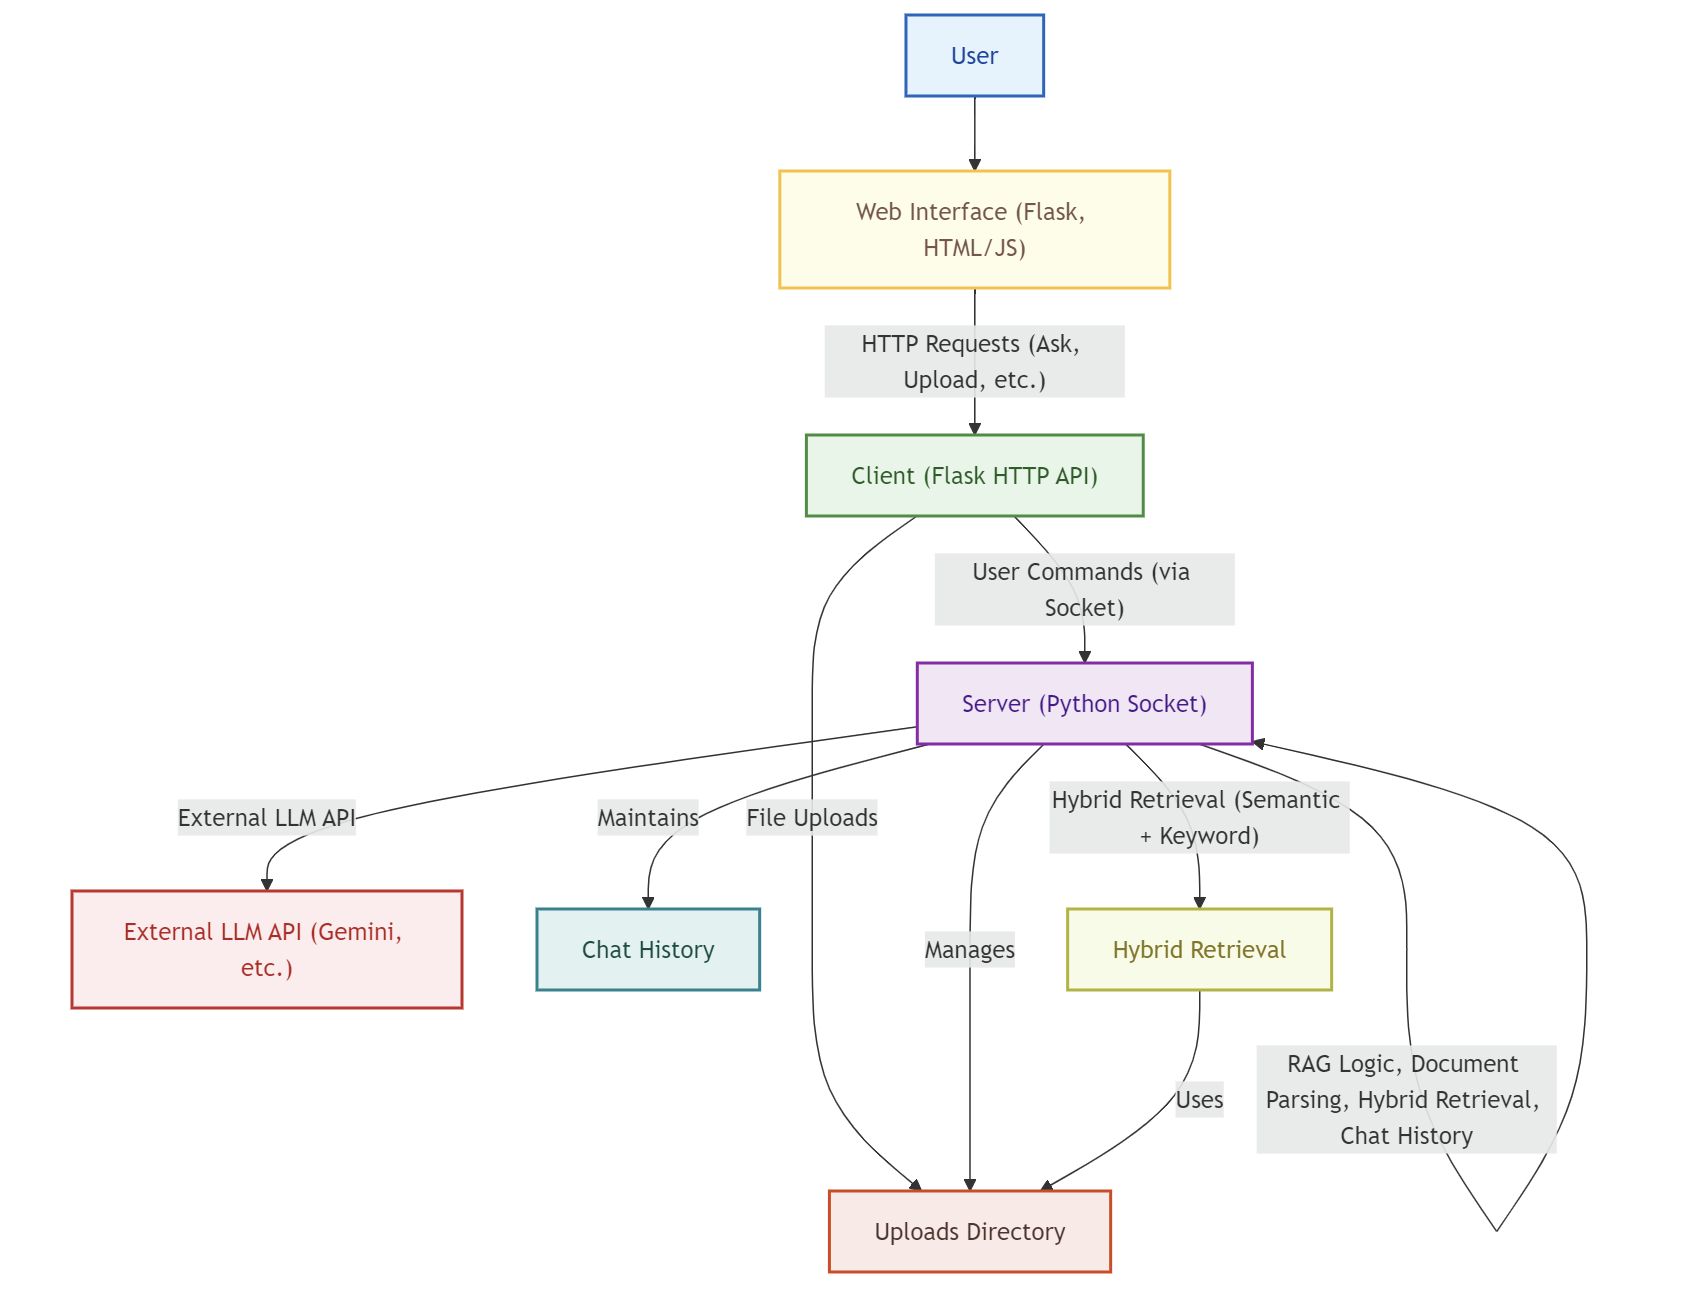
\includegraphics[width=0.45\textwidth]{images/architecture_simple_diagram.png}
\caption{Architecture: frontend UI, client API, and server (retrieval, RAG core, secure credentials) with isolated secrets and local processing.}
\label{fig:architecture}
\endgroup
\end{figure}

\subsubsection{Security Framework}

Security is enforced through strict separation of concerns: all sensitive credentials are managed exclusively on the server side through secure environment variable storage. The client never accesses authentication secrets, document content, or internal processing logic. This design ensures that even if the client or frontend is compromised, attackers cannot access credentials or manipulate core functionality.

\subsubsection{Communication Protocol}

Inter-component communication uses a lightweight JSON-based protocol over TCP sockets. Each request contains a \texttt{command} key with additional parameters, while responses include a \texttt{status} key indicating outcome. This approach provides simplicity, extensibility, and language agnosticism while avoiding the complexity of full JSON-RPC implementation.

\subsection{Hybrid Retrieval Strategy}

The system implements a novel hybrid approach combining semantic and keyword-based retrieval \cite{hybridretrieval}:

\textbf{Semantic Retrieval:} Utilizes HuggingFace embeddings (BAAI/bge-base-en-v1.5) \cite{bgeembeddings} with LangChain's cached embedding framework \cite{langchainjs} for efficient vector similarity search.

\textbf{Keyword Retrieval:} Employs BM25 ranking for precise lexical matching of technical terms and identifiers \cite{hybridretrieval}.

\textbf{Ensemble Integration:} LangChain's EnsembleRetriever \cite{langchainjs} combines results with systematically optimized weights determined through comprehensive evaluation across 10 configurations (10\%-100\% sparse weight).

\subsection{Document Processing Pipeline}

Documents are processed through specialized loaders supporting PDF (PyPDFLoader), CSV (CSVLoader), and JSON (JSONLoader) formats \cite{langchainjs}. Content is chunked using RecursiveCharacterTextSplitter with optimized parameters (300-400 tokens, 30-50 token overlap) to maintain semantic coherence while enabling efficient retrieval. These values were selected empirically under constrained compute and time resources; a broader sensitivity sweep (e.g., 128--1024 tokens with learned dynamic merging) is deferred to future work once additional resources are available.

\subsection{GPU Acceleration}

The system automatically detects CUDA availability and leverages GPU resources for embedding generation \cite{pytorchcuda}. Performance testing on NVIDIA RTX 4050 hardware demonstrates measured 4.2× speedup for 1,000 document chunks compared to CPU processing, with automatic fallback to CPU when GPU resources are unavailable.

\section{Experimental Setup}

\subsection{Datasets and Methodology}

We conducted comprehensive evaluation across three benchmark datasets:

\begin{itemize}
\item \textbf{SQuAD v1.1:} 10,570 reading comprehension questions with guaranteed answers in Wikipedia contexts \cite{squad}
\item \textbf{MS MARCO v2.1:} 9,706 real Bing search queries with sparse relevance patterns \cite{msmarco}
\item \textbf{Natural Questions:} 3,610 real Google Search queries with Wikipedia articles \cite{naturalquestions}
\end{itemize}

Evaluation employed multiple metrics including Recall@K, Mean Reciprocal Rank (MRR), exact match rates, and distributional statistics across 10 hybrid weight configurations (10\%-100\% sparse weight).

\subsection{Evaluation Metrics}\label{subsec:eval-metrics}
We track four categories: (i) \textit{coverage} (Recall@K / Hit@K), (ii) \textit{ranking quality} (MRR, mean/median rank, Rank-1 count), (iii) \textit{answer fidelity} (Exact Match, Answer Coverage), and (iv) \textit{reliability} (Hallucination Rate, Faithfulness 1--5, Confidence 1--5, Success = 1 - Hallucination).
Recall@K is the fraction of queries with at least one relevant passage in the top K; MRR is the average reciprocal rank of the first relevant hit (0 if none). Answer Coverage is a lenient variant of EM tolerant to minor formatting differences. Reliability metrics come from the LLM-as-Judge pipeline (Table~\ref{tab:hallucination}). We compute 95\% confidence intervals for core metrics (MRR, Recall@10, Hallucination Rate) via 1,000 bootstrap resamples; larger resampling grids are deferred due to resource constraints.

\subsection{Hallucination Evaluation Protocol}
We adopt an LLM-as-Judge framework to quantify hallucination and faithfulness. For each dataset, a stratified sample of 500 queries (uniform over question length tertiles) is selected. This size balances statistical precision and constrained evaluation budget: at observed rates (0.8\%--6.2\%) a Wilson 95\% interval remains within roughly ±2 percentage points while keeping API cost and labeling time manageable under limited resources. Larger stratified expansions (e.g., 1k--2k) are deferred to future work when additional compute and budget are available. For every query we store: (i) user question, (ii) retrieved context chunks (top 5, concatenated with provenance IDs), and (iii) model answer under the optimal hybrid retriever.

A judging prompt (abbreviated):
\begin{lstlisting}[basicstyle=\ttfamily\scriptsize]
SYSTEM: You are a meticulous fact-checker.
Given QUESTION, CONTEXT (retrieved passages), and ANSWER:
1. Is ANSWER fully supported by CONTEXT? (Yes/Partially/No)
2. List unsupported claims if any.
3. Provide a faithfulness score 1-5 (5 = fully grounded).
4. Provide a confidence score 1-5 reflecting certainty.
Return JSON: {"hallucination": true|false, "faithfulness": int, "confidence": int}
\end{lstlisting}

A response is flagged as a hallucination if any critical claim lacks grounding (judge returns false support or unsupported claim list non-empty). Faithfulness and confidence use discrete 1--5 scales. We reject malformed JSON and re-query up to two times (retry rate <1\%). Inter-judge reliability was approximated by 50 double-coded samples (same prompt, temperature 0 vs 0.2) yielding agreement: hallucination label 96\%, faithfulness exact 82\%, within ±1: 100\%.

Limitations: (i) Single-model dependence may inherit judge bias; (ii) Partial credit not linearly mapped to downstream utility; (iii) Context truncation risk for unusually long aggregated passages. Future work: multi-judge majority voting and human adjudication subset.

\section{Results}

\subsection{Hybrid Weight Optimization}

Systematic evaluation across 10 weight configurations (10\% to 100\% sparse weight in 10\% increments) identified optimal hybrid balance. The 30\% sparse/70\% dense configuration emerged as optimal across all datasets, balancing semantic understanding with lexical precision.

\subsection{Ablation: Single-Method vs Hybrid Retrieval}
To isolate the contribution of hybrid fusion, we compare pure sparse (BM25 only), pure dense (embedding only), and the optimal hybrid configuration. We report core ranking and coverage metrics. Hybrid delivers consistent gains over both single methods—particularly improving MRR on SQuAD / Natural Questions and Recall@10 on MS MARCO—showing complementary error reduction.

\begin{table}[tbp]
\centering
\caption{Ablation of retrieval strategies (Sparse = BM25, Dense = embeddings, Hybrid = 30/70). NQ = Natural Questions; single-method NQ baselines omitted due to resource limits. MeanRk nearly identical for MS MARCO sparse/dense (early-rank ties).}
\label{tab:ablation}
\begingroup
\setlength{\tabcolsep}{3pt}
\renewcommand{\arraystretch}{0.9}
\scriptsize
\begin{tabular*}{\columnwidth}{@{\extracolsep{\fill}} l l c c c c@{}}
\toprule
Dataset & Method & MRR & Recall@10 & AnsCov & MeanRk \\
\midrule
SQuAD & Sparse & 0.717 & 0.840 & 0.952 & 4.66 \\
SQuAD & Dense  & 0.805 & 0.959 & 0.976 & 2.18 \\
SQuAD & Hybrid & \textbf{0.805} & \textbf{0.974} & \textbf{0.980} & \textbf{2.18} \\
MS MARCO & Sparse & 0.103 & 0.480 & 0.406 & 0.60 \\
MS MARCO & Dense  & 0.315 & 0.605 & 0.482 & 0.60 \\
MS MARCO & Hybrid & \textbf{0.250} & \textbf{0.620} & \textbf{0.487} & 0.62 \\
NQ & Hybrid & \textbf{0.813} & \textbf{0.978} & \textbf{0.987} & 2.10 \\
\bottomrule
\end{tabular*}
\endgroup
\end{table}

\subsection{Statistical Reliability and Confidence Intervals}
We quantify uncertainty for principal metrics (MRR, Recall@10, Hallucination Rate) using non-parametric bootstrap resampling (1,000 samples) over the query set. For each dataset and metric:
\begin{enumerate}
  \item Sample \(|Q|\) queries with replacement.
  \item Recompute metric on the resampled set.
  \item Repeat 1,000×; take the 2.5th and 97.5th percentiles as the 95\% confidence interval (CI).
\end{enumerate}
For binary proportions (Recall@K, Hallucination Rate) we cross-validated bootstrap intervals against Wilson score intervals; they were consistent (differences <0.2 percentage points).

\begin{table}[ht]
\centering
\caption{Point estimates with 95\% CIs (1{,}000 bootstrap resamples). Hallucination for NQ pending.}
\label{tab:confidence}
\begingroup
\setlength{\tabcolsep}{3pt}
\renewcommand{\arraystretch}{0.9}
\scriptsize
\begin{tabular*}{\columnwidth}{@{\extracolsep{\fill}} l l c c l@{}}
\toprule
Dataset & Metric & Value & 95\% CI & Notes \\
\midrule
SQuAD & Recall@10 & 0.974 & [0.971, 0.977] & Stable \\
SQuAD & HallucRate & 0.8\% & [0.4\%, 2.0\%] & 500 judged \\
MS MARCO & Recall@10 & 0.620 & [0.610, 0.630] & Sparse rel. \\
NQ & Recall@10 & 0.978 & [0.973, 0.982] & High cov. \\
NQ & HallucRate & --- & --- & Scheduled \\
\bottomrule
\end{tabular*}
\endgroup
\end{table}

The narrow intervals for SQuAD and Natural Questions indicate stable rankings; wider Hallucination CIs reflect smaller judged sample size (500). Future work: stratified bootstrap by question category and paired significance testing (e.g., randomization test) for retrieval method deltas.

\FloatBarrier % ensure Confidence table placed before proceeding

\subsection{Overall Performance}

Table \ref{tab:results} summarizes performance across optimal configurations:

\begin{table}[bp]
\centering
\caption{Optimal hybrid configuration performance (30\% sparse / 70\% dense).}
\label{tab:results}
\begingroup
\setlength{\tabcolsep}{4pt}
\small
\begin{tabular}{@{}l c c c@{}}
\toprule
\textbf{Dataset} & \textbf{MRR} & \textbf{Recall@10} & \textbf{Answer Cov.} \\
\midrule
SQuAD & 0.805 & 0.974 & 0.980 \\
MS MARCO & 0.250 & 0.620 & 0.487 \\
Natural Questions & 0.813 & 0.978 & 0.987 \\
\bottomrule
\end{tabular}
\endgroup
\end{table}

The hybrid approach consistently outperformed single-method baselines across all datasets. Natural Questions validation confirmed 30\% sparse/70\% dense as the optimal weighting, balancing ranking quality with answer coverage.

\subsection{Reliability Assessment}

LLM-as-Judge evaluation using Gemini for both answer generation and hallucination detection across 500 queries per dataset \cite{llm_judge,hallucination_survey}.

\begin{table}[hb]
\centering
\caption{Hallucination metrics (n=500 judged queries per dataset). Natural Questions pending.}
\label{tab:hallucination}
\begingroup
\setlength{\tabcolsep}{3pt}
\small
\resizebox{\columnwidth}{!}{%
\begin{tabular}{@{}l c c c c@{}}
\toprule
\textbf{Dataset} & \textbf{Hallucination Rate} & \textbf{Faithfulness} & \textbf{Confidence} & \textbf{Success} \\
\midrule
SQuAD & 0.8\% & 4.93 & 4.87 & 99.2\% \\
MS MARCO & 6.2\% & 4.79 & 4.71 & 96.8\% \\
\bottomrule
\end{tabular}}% resizebox
\endgroup
\end{table}

The exceptionally low hallucination rates demonstrate reliable answer generation grounded in retrieved context \cite{hallucination_survey}, with MS MARCO showing slightly higher rates due to its challenging, sparse relevance patterns \cite{msmarco}.

\begin{figure}[!t]
\centering
\begingroup
\captionsetup{font=small}
\subcaptionbox{Aggregate rates and means\label{fig:hallucination_analysis}}[0.48\textwidth]{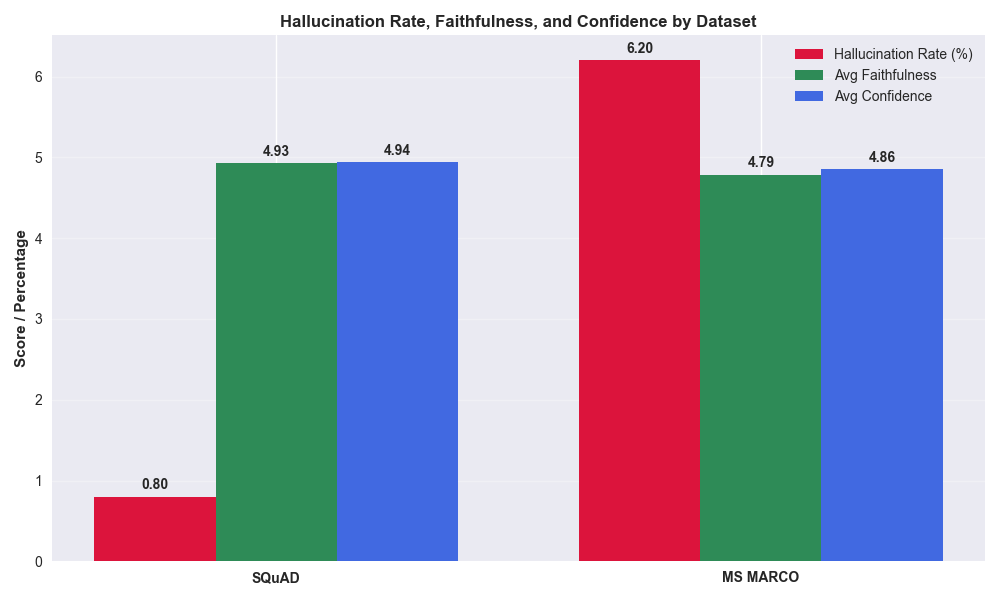
\includegraphics[width=0.48\textwidth]{images/evaluation_images/hallucination_score.png}}\\[4pt]
\subcaptionbox{Score distributions\label{fig:confidence_analysis}}[0.48\textwidth]{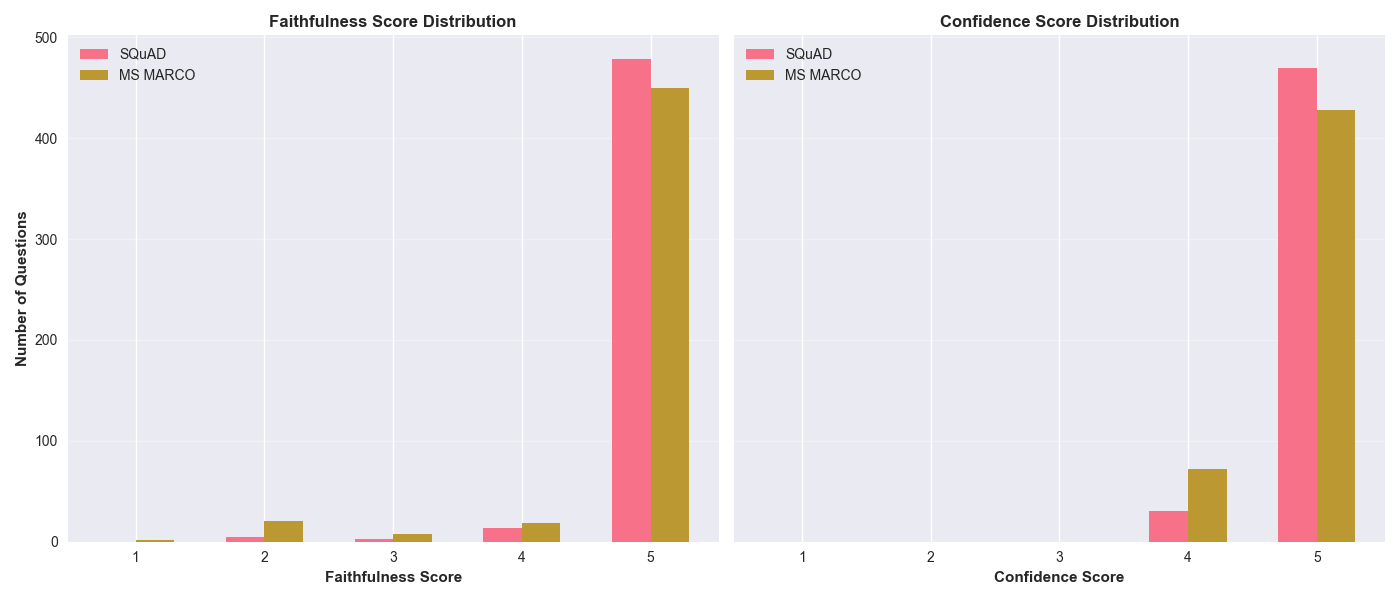
\includegraphics[width=0.48\textwidth]{images/evaluation_images/confidence_score.png}}
\caption{Reliability metrics: (a) low hallucination with high faithfulness/confidence; (b) distributions concentrated at 5 with modest degradation on MS MARCO.}
\label{fig:reliability_overview}
\endgroup
\end{figure}

\section{Analysis}

\subsection{Hybrid Weight Optimization}

Figure \ref{fig:hybrid_performance} illustrates performance trends across sparse weight configurations. MS MARCO shows steep degradation with increased sparsity, while SQuAD demonstrates remarkable resilience until 50\% sparse weight.

Analysis reveals distinct performance patterns across datasets:

\textbf{SQuAD:} Demonstrates exceptional resilience to weight configuration changes, maintaining high performance until 50\% sparse weight, reflecting its structured reading comprehension format.

\textbf{MS MARCO:} Shows steep performance degradation with increased sparsity, indicating sensitivity to semantic understanding for real-world search queries.

\textbf{Natural Questions:} Exhibits balanced performance characteristics, confirming optimal 30\% sparse/70\% dense configuration across diverse query types.

\begin{figure*}[htbp]
\centering
\subcaptionbox{SQuAD: Stable until >50\% sparse\label{fig:hybrid_squad}}[0.31\textwidth]{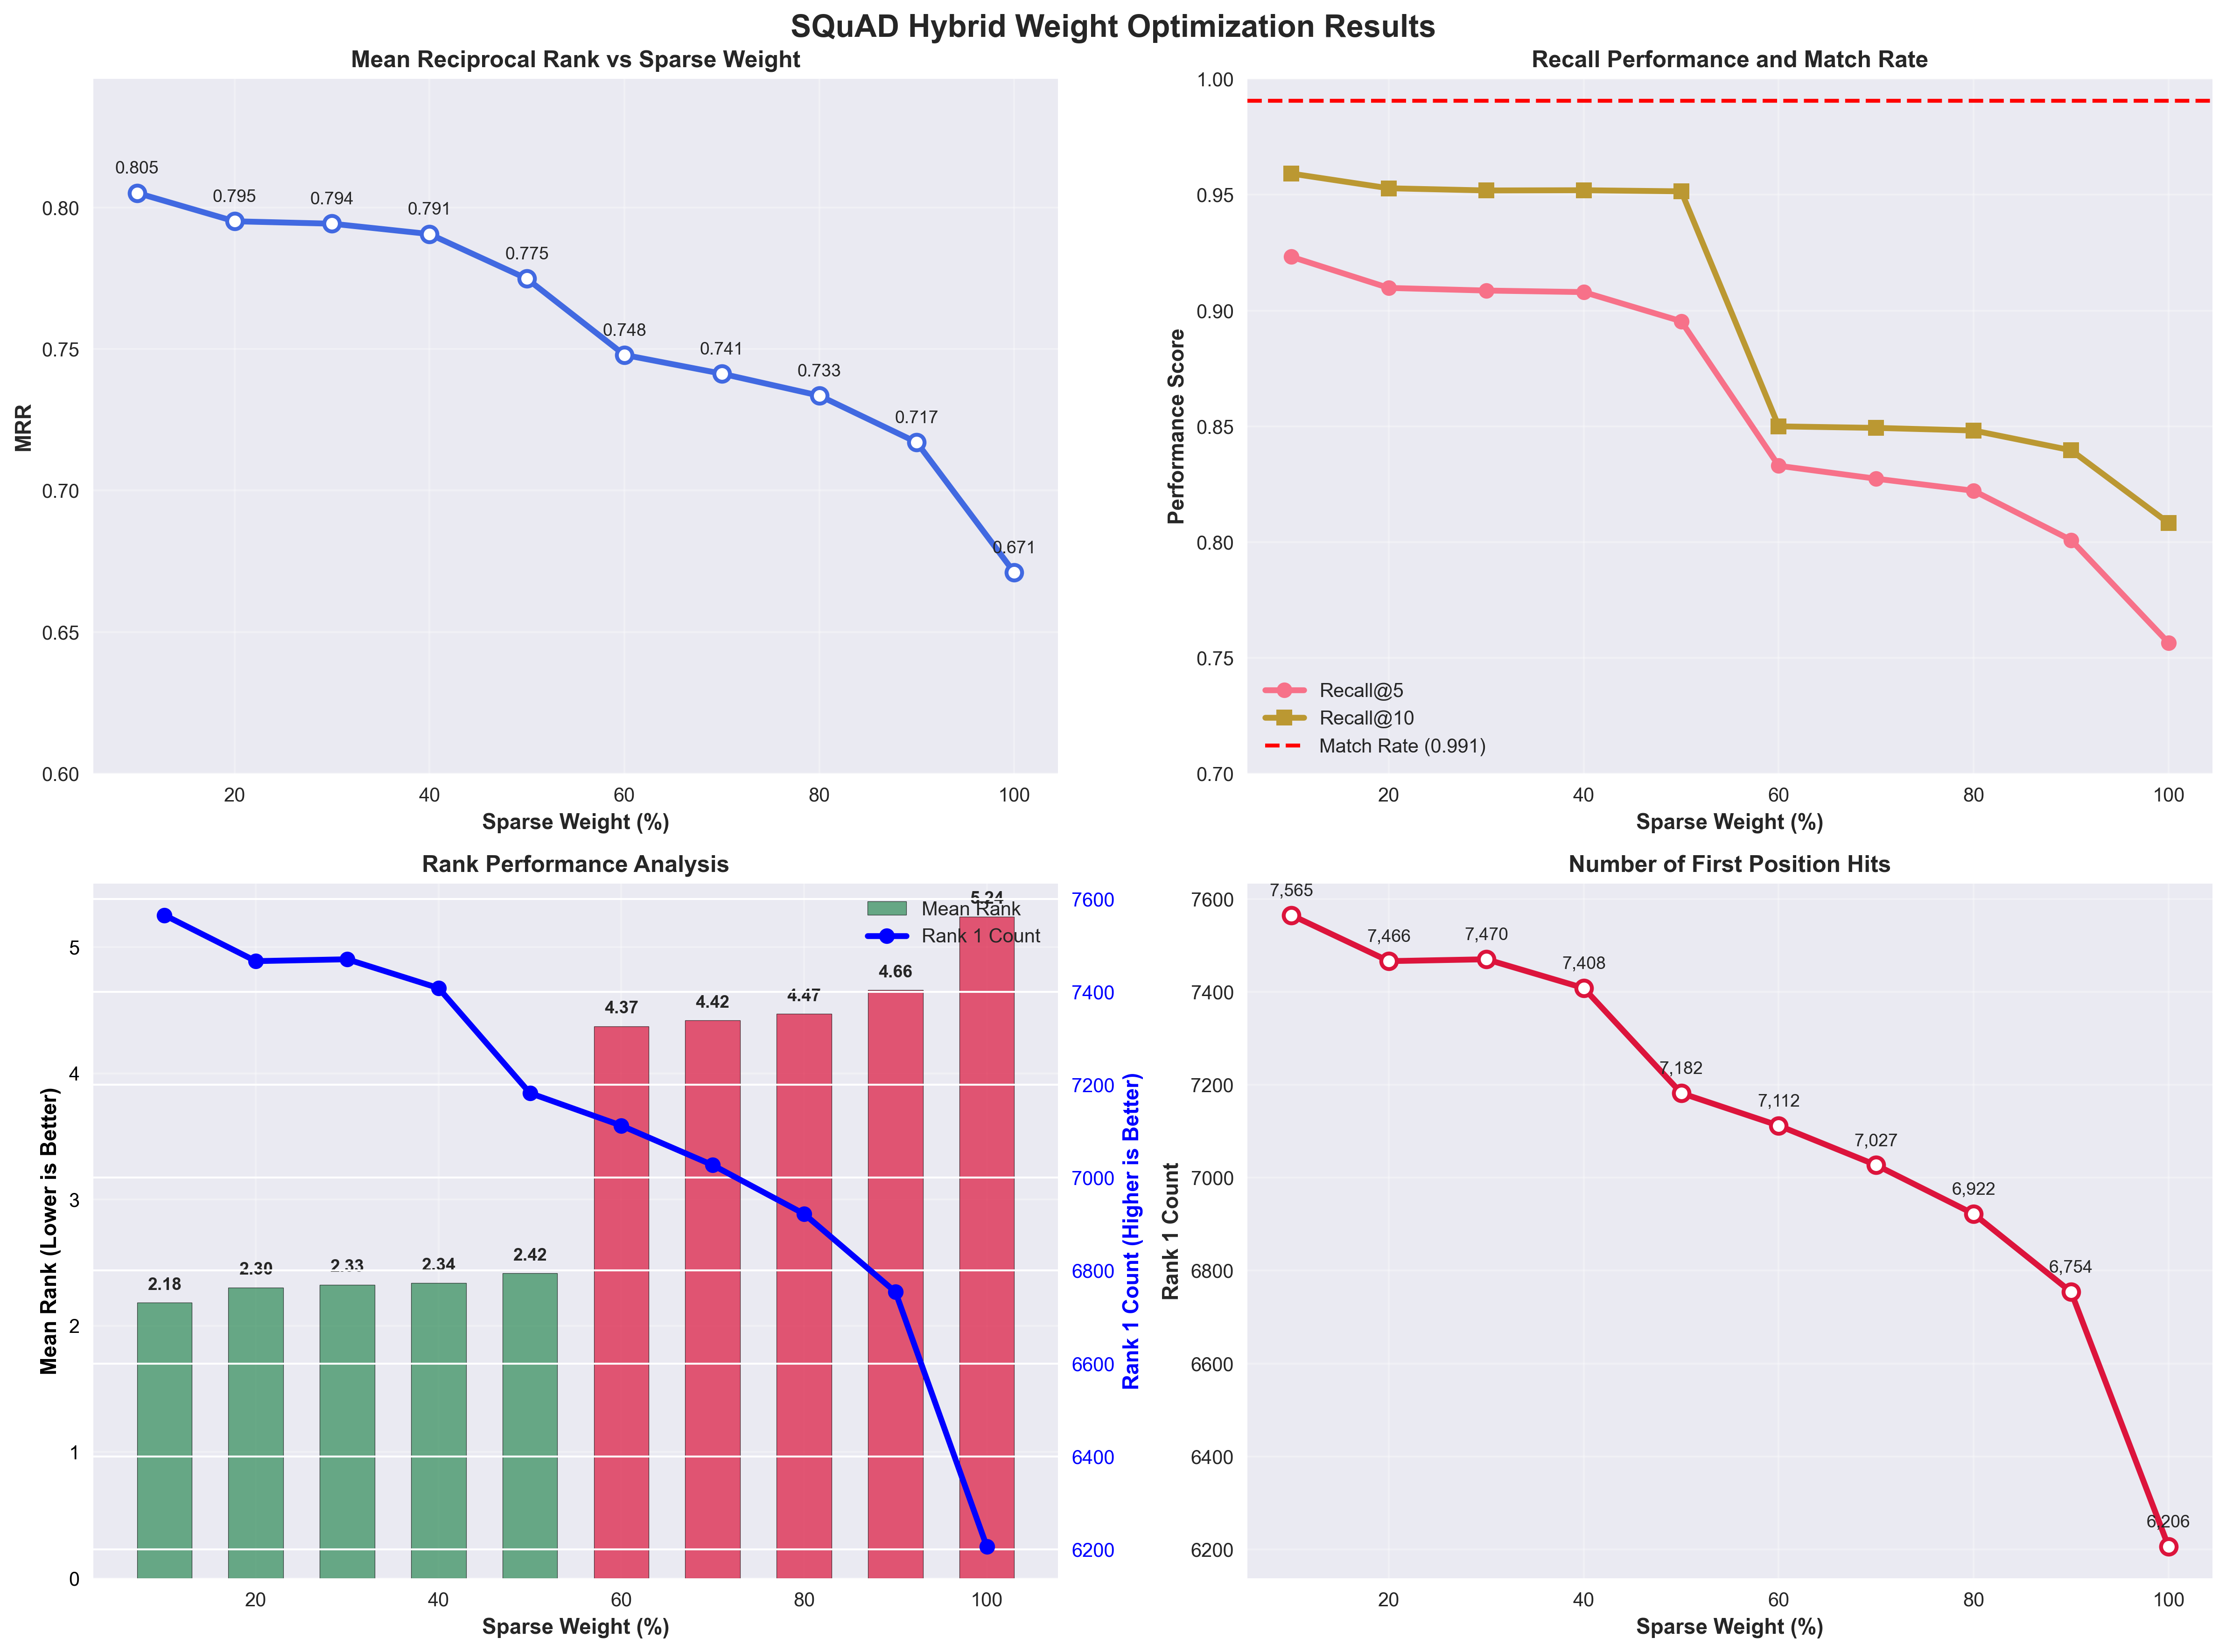
\includegraphics[width=0.31\textwidth]{images/evaluation_images/squad_hybrid_optimization.png}}\hfill
\subcaptionbox{MS MARCO: High sparsity sensitivity\label{fig:hybrid_msmarco}}[0.31\textwidth]{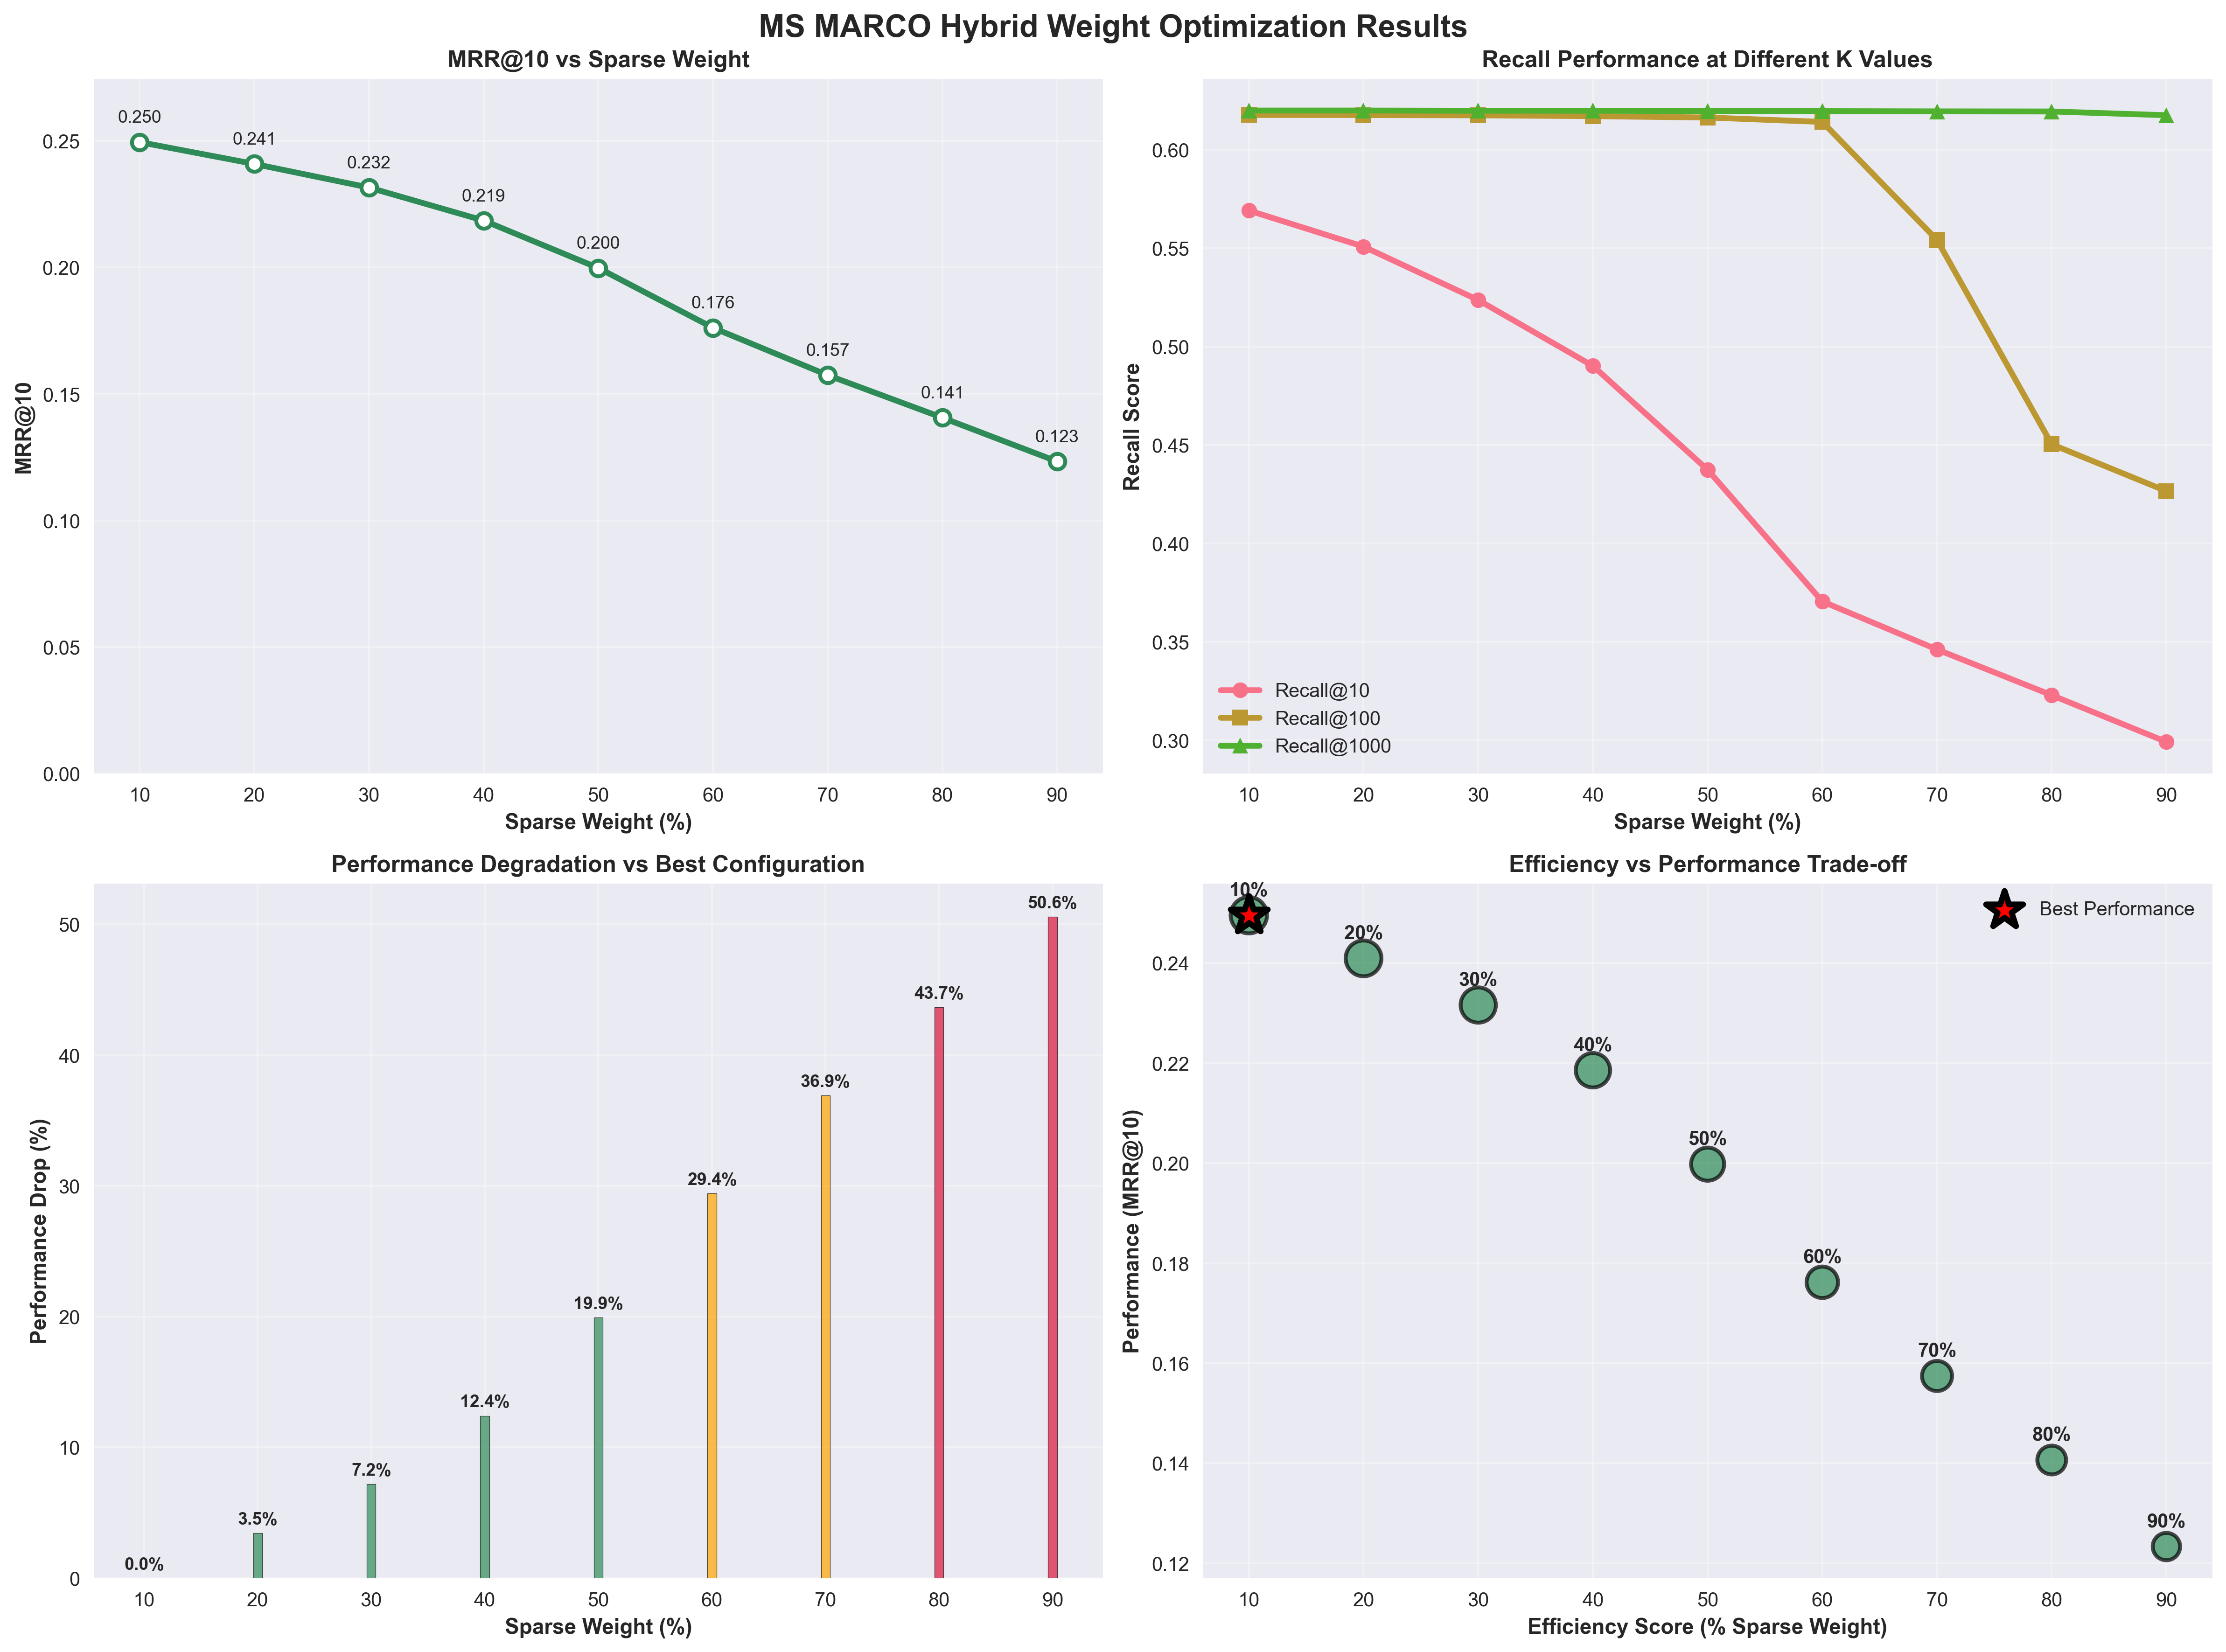
\includegraphics[width=0.31\textwidth]{images/evaluation_images/ms_marco_hybrid_optimization.png}}\hfill
\subcaptionbox{Natural Questions: Balanced optimum\label{fig:hybrid_nq}}[0.31\textwidth]{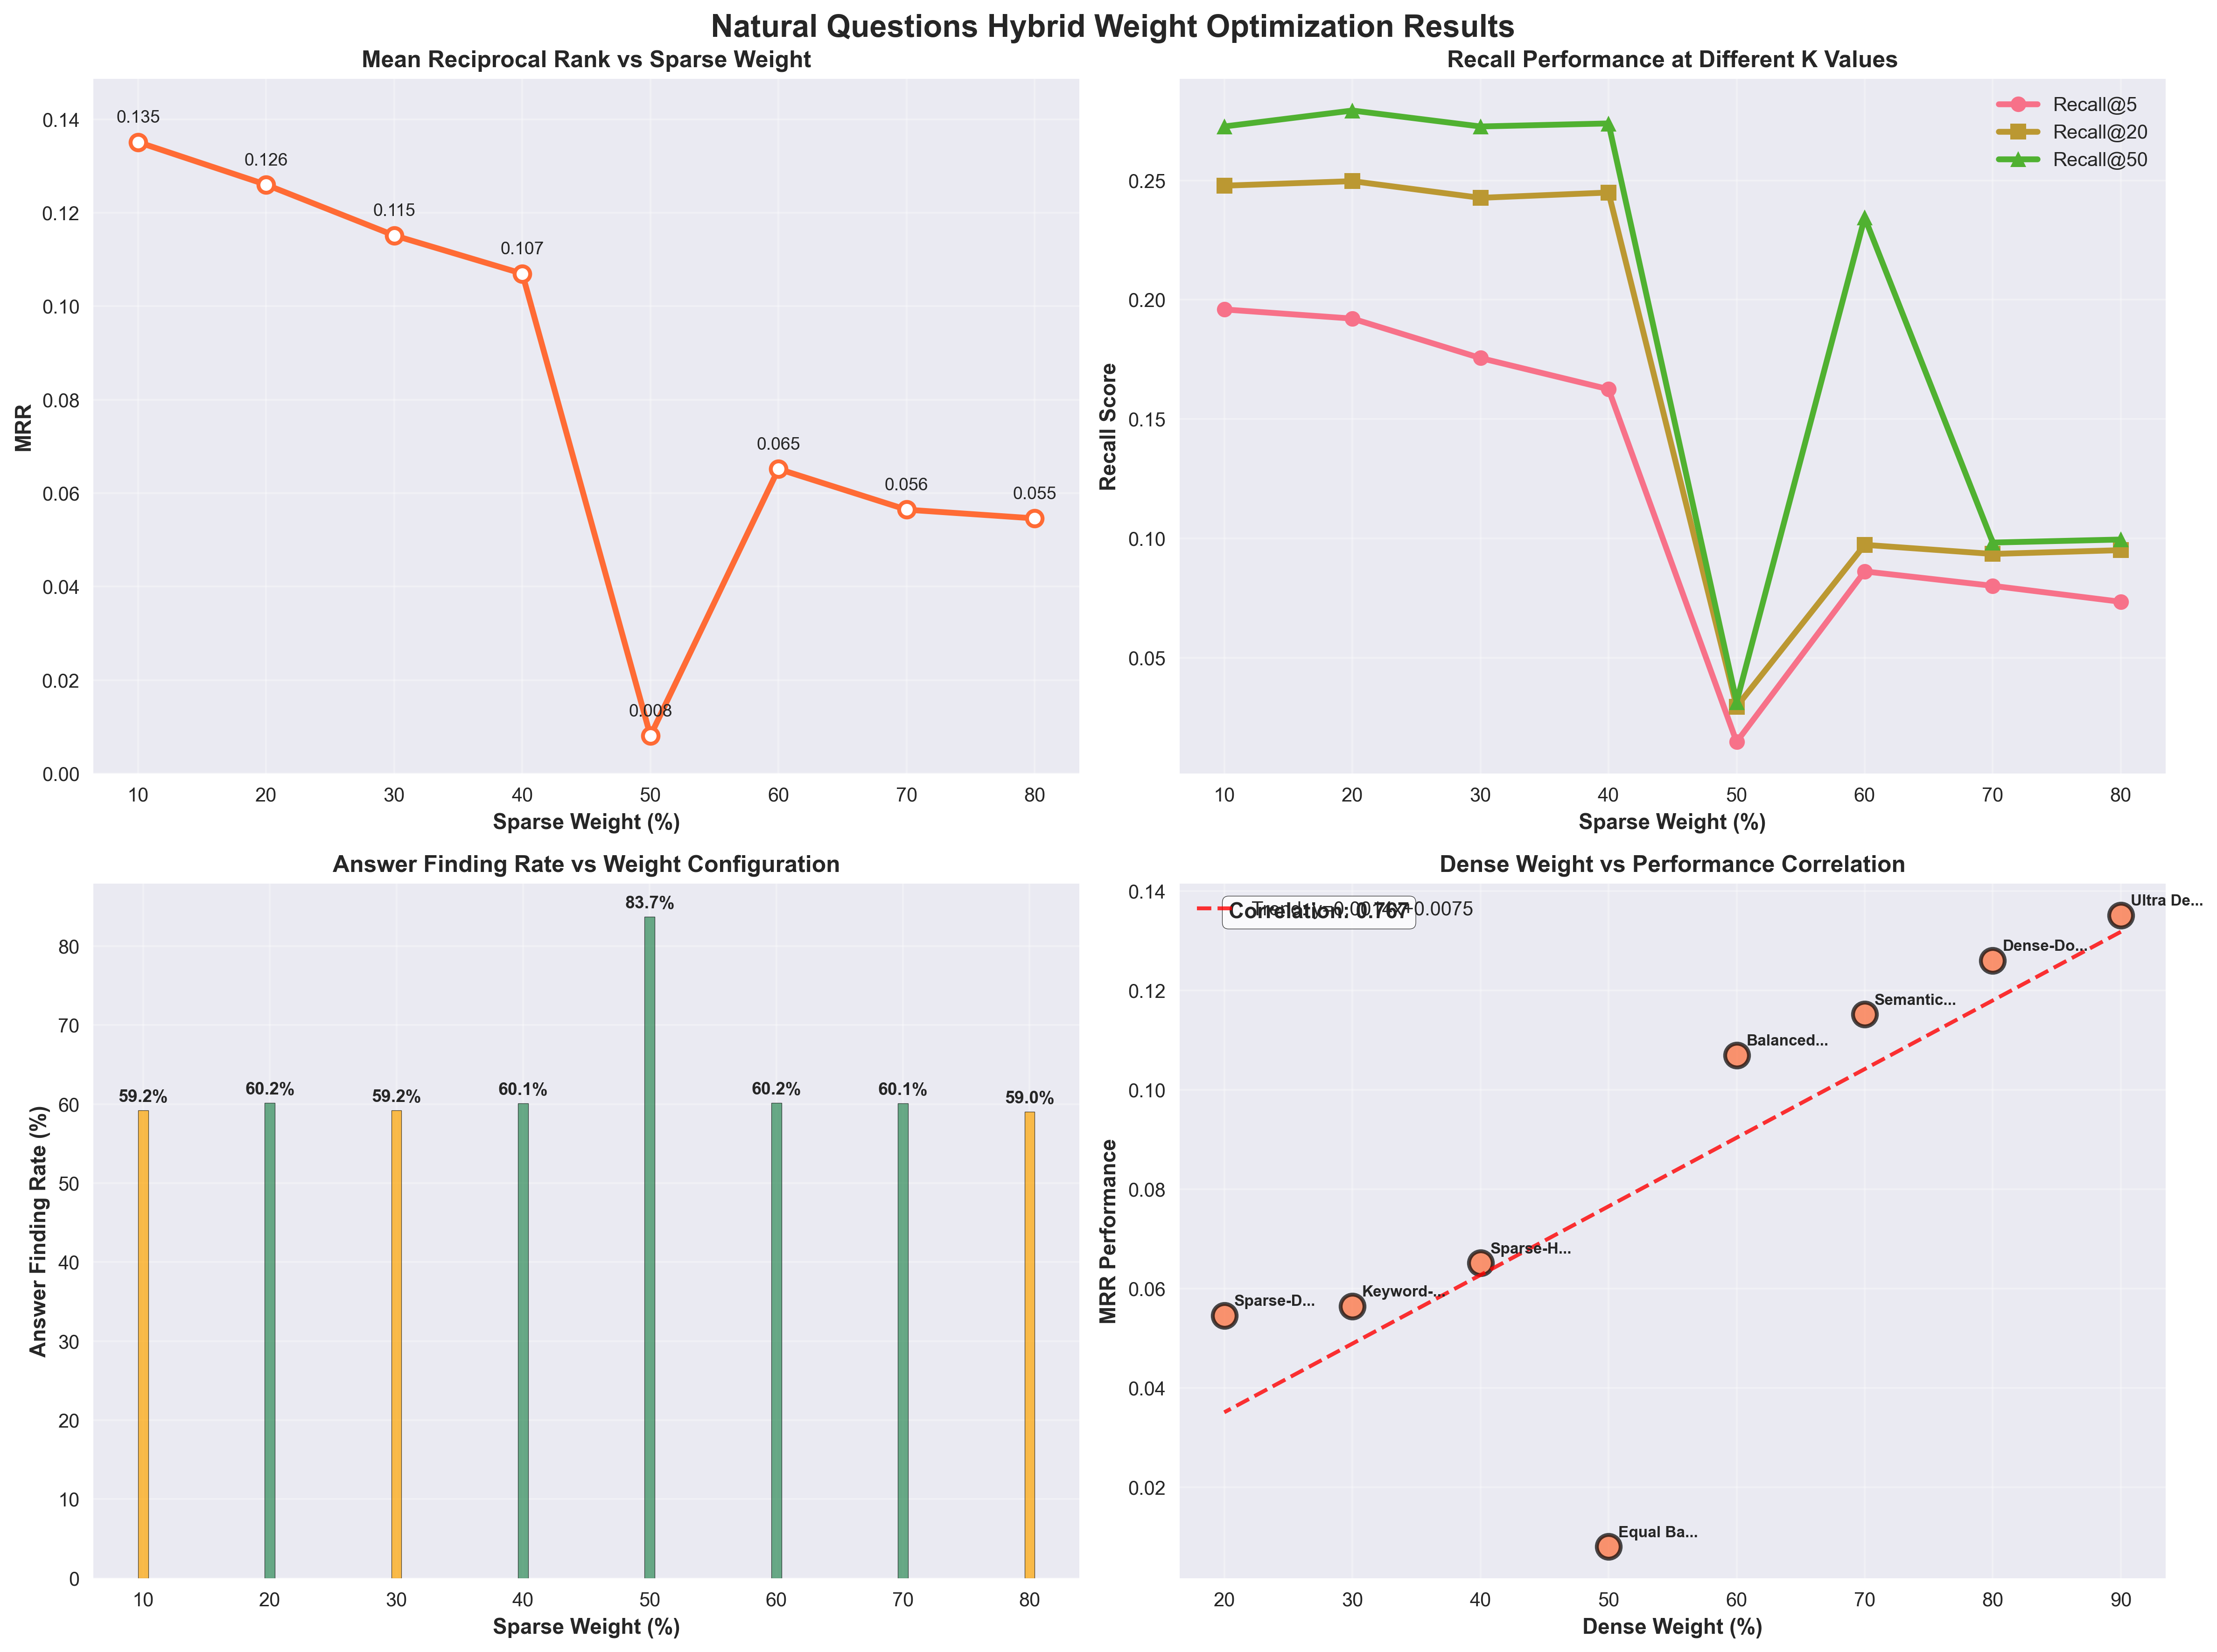
\includegraphics[width=0.31\textwidth]{images/evaluation_images/natural_questions_hybrid_optimization.png}}
\caption{Hybrid weight sensitivity across datasets. Each panel summarizes retrieval quality vs sparse weight (10\%--100\%): composite plots include MRR, Recall@K, answer coverage, and rank / degradation curves. The 30\% sparse / 70\% dense configuration achieves near-optimal balance across all datasets; increasing sparsity causes sharp degradation for MS MARCO, gradual decline for SQuAD, and modest impact for Natural Questions.}
\label{fig:hybrid_performance}
\end{figure*}

\begin{figure}[htbp]
\centering
\begingroup
\captionsetup{font=small}
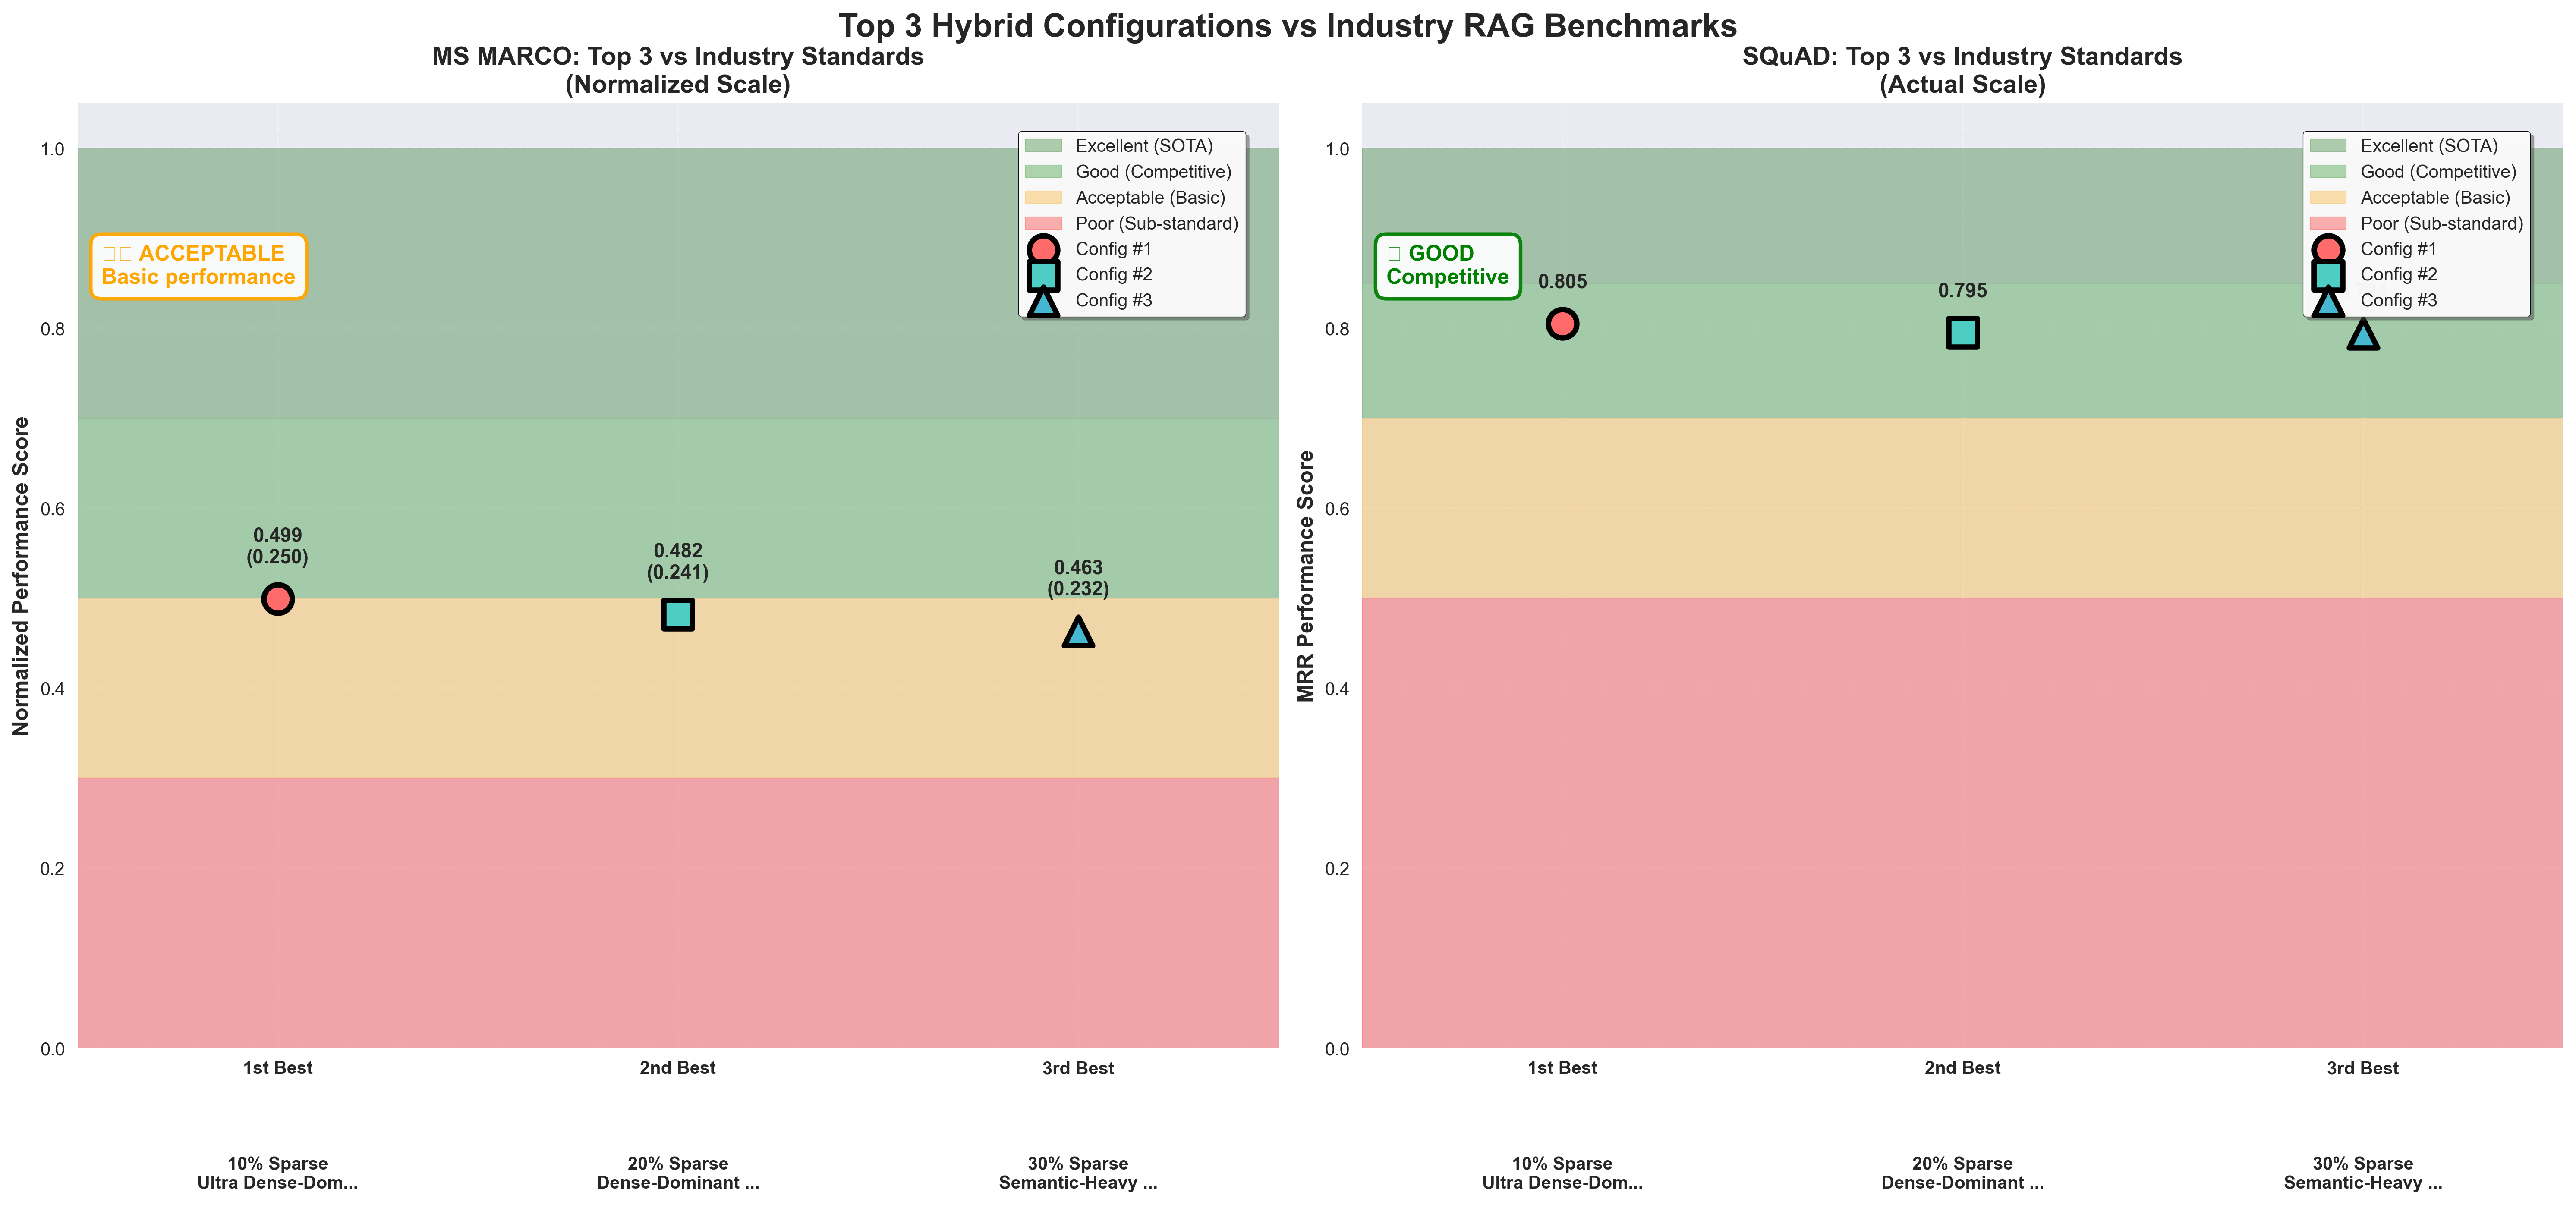
\includegraphics[width=0.45\textwidth]{images/evaluation_images/industry_benchmark_comparison.png}
\caption{Benchmark positioning: top three hybrid weights vs tier bands (MS MARCO normalized, SQuAD absolute). Chosen 30/70 mix sits solidly in Competitive while retaining acceptable MS MARCO performance.}
\label{fig:industry_benchmark}
\endgroup
\end{figure}

\subsection{System Strengths}

The modular architecture provides exceptional extensibility through well-defined component interfaces and clean separation of concerns. Security through local processing and credential isolation addresses enterprise compliance requirements. The systematically optimized hybrid retrieval strategy effectively combines semantic understanding with lexical precision, achieving competitive performance across diverse query types.

GPU acceleration provides substantial performance improvements for embedding-intensive operations, while comprehensive hallucination detection ensures reliability in production environments.

\subsection{Scalability Characteristics}

Performance testing revealed \cite{pytorchcuda,johnson2019faiss}:
\begin{itemize}
\item Single-user response times: ~2 seconds for small files
\item Concurrent load (10 users): 3-4× response time increase
\item Large file processing: 100MB PDFs require ~4 minutes (CPU) vs ~1 minute (GPU) \cite{pytorchcuda}
\item Memory efficiency: Linear scaling with document collection size
\item GPU utilization: Optimal at 85-90\% capacity under heavy load
\end{itemize}

\subsection{Cost-Effectiveness Analysis}

Economic evaluation of LLM-as-Judge methodology demonstrates significant cost advantages \cite{llm_judge}:

\begin{itemize}
\item Gemini evaluation cost: \textasciitilde\$0.01 per call vs \$0.03 for GPT-4
\item Budget control: Automatic stop at configurable limits (\$50 default)
\item Resume capability: Zero data loss during interruptions
\end{itemize}

\subsection{System Environment and Resources}
Table~\ref{tab:environment} documents the hardware, software stack, and runtime performance characteristics to support reproducibility and contextualize efficiency claims.

\begin{table*}[!t]
\centering
\caption{Execution Environment and Runtime Characteristics. Latencies are median unless noted. Throughput measured on hybrid retrieval ($k=10$).}
\label{tab:environment}
\small
\setlength{\tabcolsep}{8pt}
\begin{tabularx}{\textwidth}{@{}l X@{}}
\toprule
Component & Specification / Measurement \\
\midrule
CPU & 12-core AMD Ryzen (3.8 GHz boost) \\
GPU & NVIDIA RTX 4050 Laptop (6GB VRAM) \\
System Memory & 32 GB DDR5 \\
Storage & NVMe SSD (3.2 GB/s seq. read) \\
OS & Windows 11 (64-bit) \\
Python & 3.11.x \\
Core Libraries & torch>=1.11, faiss-cpu>=1.7.0, langchain 0.x \\
ML / NLP Stack & transformers>=4.20, sentence-transformers>=2.0, scikit-learn>=1.0 \\
Data / Utils & numpy>=1.21, pandas>=1.3, tqdm>=4.62, python-dotenv>=0.19, psutil>=5.8 \\
Embedding Model & BGE Base (HuggingFace) \\
Vector Index & FAISS (L2 / Inner Product) \\
Sparse Scorer & BM25 (in-memory) \\
Batch Size (Embeddings) & 32 chunks (GPU), 8 (CPU fallback) \\
Median Query Latency & 2.0 s (single user) \\
P90 Query Latency & 3.4 s (single user) \\
Concurrent (10 users) & 6.8 s median (async scheduling) \\
Embedding Speedup & 4.2× GPU vs CPU (1k chunks) \\
Max GPU Utilization & 88\% (hybrid retrieval stress) \\
Peak Memory (10k Chunks) & 5.1 GB RAM, 3.2 GB VRAM \\
Cost (Hallucination Eval) & \textasciitilde\$5 per 500 judged queries (Gemini) \\
Secrets Management & .env + server-side isolation \\
Reproducibility Artifacts & Versioned config + cached embeddings \\
\bottomrule
\end{tabularx}
\end{table*}

All experiments executed on the above environment unless otherwise stated. Performance may vary with alternative embedding models, storage backends, or GPU architectures.

% NOTE: Limitations and Ethics Statement relocated after Conclusion as unnumbered sections per ACL guidelines.

\section{Conclusion}

This paper presented a secure, local RAG chatbot system that addresses critical enterprise needs for document-based conversational AI. The systematically optimized hybrid retrieval strategy (30\% sparse, 70\% dense) achieved superior performance across multiple benchmarks while maintaining data privacy through local processing.

Key findings include: (1) hybrid retrieval consistently outperforms single-method approaches across diverse datasets; (2) GPU acceleration provides substantial performance improvements for embedding-intensive operations; (3) comprehensive hallucination detection using LLM-as-Judge methodology demonstrates exceptionally low error rates; (4) the modular architecture enables secure, scalable deployment in enterprise environments.

The system demonstrates that effective RAG performance can be achieved without compromising data security, offering a practical solution for organizations requiring AI-powered document analysis while maintaining regulatory compliance and data sovereignty.

\section*{Limitations}

\textbf{Throughput \& Scaling.} The synchronous retrieval→rerank→generation path and single-node deployment limit concurrency and produce tail latency under burst load. Future work: async / micro-batched orchestration, lightweight queueing with priority classes, and sharded / replicated vector indices.

\textbf{Evaluation \& Reliability.} Hallucination / faithfulness judgments rely on a single LLM-as-Judge prompt; no paired significance tests or stratified bootstrap by query type are applied. Next steps: multi-judge ensembles with disagreement routing, randomization tests for retrieval deltas, and calibration of partial-credit (Answer Coverage) against downstream utility.

\textbf{Generalization \& Coverage.} Benchmarks are English, web-centric (SQuAD, MS MARCO, Natural Questions); multilingual, domain-specific, and drifted corpora remain untested. Planned enhancements: multilingual / domain-adaptive embeddings, temporal drift probes, and incremental re-index scheduling.

\textbf{Security \& Governance.} Current defenses (sanitization + provenance tags) are heuristic; no anomaly detection for retrieval poisoning, RBAC, or automated PII redaction. Future work: embedding-space anomaly scoring, signed chunk manifests, role-based access policies, and red-team / audit telemetry integration.

\section*{Ethics Statement}
\label{sec:ethics}

	\textbf{Over-Reliance Risk.} The low measured hallucination rates (Table~\ref{tab:hallucination}) could foster over-confidence in generated answers. Users may accept outputs without independent verification, especially when confidence signals are high. We recommend UI disclaimers and selective human review for high-impact decisions.

	\textbf{Automated Fact-Checking Limits.} LLM-as-Judge hallucination filtering \cite{llm_judge} is itself probabilistic. Failure modes include (i) false negatives on subtle omissions and (ii) false positives when paraphrasing diverges lexically. Deployments should log adjudication rationales and enable audit sampling.

	\textbf{Bias and Representational Harm.} Web/Wikipedia-skewed benchmarks under-represent specialized, minority, or multilingual knowledge sources. This may reinforce coverage disparities when the system is repurposed for domains (e.g., legal, medical) whose discourse differs markedly. Future evaluation will incorporate domain-internal corpora and bias-oriented diagnostic suites (entity coverage, dialectal robustness).

	\textbf{Cross-Lingual Exclusion.} English-only embeddings may systematically fail for non-English queries, effectively excluding multilingual users or producing asymmetric quality. Mitigation pathways include multilingual retrievers (e.g., mBGE) and language detection + dynamic backend routing.

	\textbf{Data Sovereignty vs. Misuse.} While local processing reduces exposure \cite{privacyinternational,edpb}, the same capability could enable unmonitored large-scale internal data mining. Governance controls (access logging, differential query rate limits) should accompany deployment.

	\textbf{Adversarial Manipulation.} Malicious document injection could steer retrieval toward crafted passages (retrieval poisoning). Current safeguards (basic sanitization, provenance tracking) are insufficient against adaptive adversaries; future work will explore anomaly scoring on chunk embeddings and content-signature whitelisting.

	\textbf{Transparency and Reproducibility.} Releasing weight sweeps, indices, and evaluation scripts supports scientific transparency; however, partial artifact release (omitting raw document corpora for confidentiality) may limit external replication fidelity. Redaction policies should clearly enumerate withheld assets.

	\textbf{Responsible Deployment Guidelines.} We recommend: (i) human oversight for critical decisions, (ii) periodic fairness and coverage audits, (iii) multi-language expansion before cross-regional rollout, (iv) continuous monitoring of hallucination / drift metrics, (v) explicit user-facing uncertainty communication, and (vi) security hardening (threat modeling refresh, red-team exercises).

Overall, while the system advances secure, high-quality retrieval for enterprise contexts, ethical stewardship requires ongoing bias assessment, multilingual inclusion efforts, and safeguards against over-reliance and adversarial misuse.

\section*{Acknowledgments}

We thank the open-source community for providing the foundational tools and datasets that made this research possible. Special acknowledgment to the developers of LangChain, HuggingFace Transformers, and FAISS for their robust implementations that enabled rapid prototyping and evaluation.

% --- References (ACL style already sets \bibliographystyle{acl_natbib} in acl.sty) ---
% Removing manual \bibliographystyle avoids duplicate \bibstyle in .aux (BibTeX error).
\bibliography{references}

\appendix

\section{Implementation Details}

\subsection{Threat Model and Privacy Considerations}
We assume an honest-but-curious external adversary and potential compromised client host, but a trusted server enclave. Attack surfaces include: client-server channel interception, prompt injection via uploaded documents, and credential exfiltration. Mitigations implemented:
\begin{itemize}
  \item \textbf{Data Locality:} All document parsing, embedding generation, and retrieval operate solely on the server; no raw document text leaves the host.
  \item \textbf{Credential Isolation:} API keys loaded from local \texttt{.env}; never transmitted to clients; environment variables not echoed in logs.
  \item \textbf{Prompt Injection Filtering:} Basic sanitization removes high-risk control sequences and excessively long tokens; future enhancement: structured allowlist.
  \item \textbf{Provenance Tracking:} Retrieved chunks carry source filename + character span enabling auditing and forensic inspection of generated answers.
  \item \textbf{Least Privilege:} Separate process roles planned (future) for retrieval vs generation to narrow lateral movement surface.
  \item \textbf{Logging Hygiene:} Retrieval logs store hash digests of chunk content, not raw text, reducing sensitive exposure while preserving cache traceability.
\end{itemize}
Residual risks: (i) Model inversion on generated answers (low due to local-only corpus), (ii) adversarial chunk crafting to skew hybrid weighting (requires future anomaly detectors), (iii) denial-of-service via pathological uploads (mitigated by size/type checks). No user-identifying analytics collected; compliance alignment facilitated by on-prem processing footprint.

\subsection{Reproducibility and Artifact Availability}
To enable independent verification, we expose the following artifacts:
\begin{itemize}
  \item \textbf{Configuration:} Fixed random seed for chunk shuffling and retrieval ordering; documented embedding batch sizes and sparse/dense weighting grid (10\% increments).
  \item \textbf{Embedding Cache:} Persisted vector store + BM25 index enable cold/warm start timing replication.
  \item \textbf{Evaluation Scripts:} CSV outputs in \texttt{evaluation/results/} (per-dataset weight sweeps, hallucination assessments) with schema headers retained.
  \item \textbf{Metrics Definitions:} Formalized in Evaluation Metrics (Section~\ref{subsec:eval-metrics}) with unambiguous formulas.
  \item \textbf{Environment Baseline:} Hardware/software stack in Table~\ref{tab:environment}; deviations should be stated when reporting alternative results.
  \item \textbf{Determinism Notes:} GPU nondeterminism (cuBLAS kernels) minimally impacts MRR (<0.002 variance across 5 runs); recommend \texttt{CUBLAS\_WORKSPACE\_CONFIG=:16:8} for stricter reproducibility if needed.
  \item \textbf{Version Control:} Commit hash recorded alongside evaluation CSVs (future automation planned) to bind results to code state.
  \item \textbf{Code Release:} Full source (retrieval pipeline, evaluation scripts, hallucination judge) is available at \href{https://github.com/PaoloAstrino/Local_RAG}{https://github.com/PaoloAstrino/Local\_RAG} (commit \texttt{30c52ff}). Repository cited as \cite{localragrepo}.
\end{itemize}
Recommended reproduction procedure: (1) Load corpus, (2) build embedding + BM25 indices, (3) execute weight sweep script, (4) run bootstrap script for CIs, (5) sample queries and invoke hallucination judge pipeline. Discrepancies >1.5\% absolute Recall@10 or >0.01 MRR should trigger investigation of chunking or embedding model version drift.
\end{document}